\documentclass[serif,8pt]{beamer}
\usetheme{default} % You can change the theme here
\usecolortheme{metropolis} % You can change the color theme here

% Packages for additional functionality
\usepackage{graphicx} % For including images
\usepackage{amsmath} % For mathematical symbols and equations
\usepackage{subfig}

% /home/bogfootlj/.local/share/fonts/NerdFonts
% Setting up fonts

\graphicspath{{./Images/}} % Where to take images from
\setbeamertemplate{section in toc}[sections numbered]
\setbeamertemplate{subsection in toc}[subsections numbered]

% Define the style for the footer with page numbers
\setbeamercolor{footline}{fg=black}
% \addtobeamertemplate{navigation symbols}{}{%
%     \usebeamerfont{footline}%
%     \usebeamercolor[fg]{footline}%
%     \hspace{1em}%
%     \insertframenumber/\inserttotalframenumber
% }

% Define a command to exclude the page counter from the first two slides
\newcommand{\noPageNumber}{%
    \setbeamertemplate{footline}{}%
}

% Define a command to reset the page counter and start numbering from the third slide
\newcommand{\resetPageNumber}{%
    \setbeamertemplate{footline}{%
        \begin{beamercolorbox}[wd=\paperwidth,ht=0.5ex,dp=1ex]{foot}%
            \hspace*{1em}\hfill \insertframenumber/\inserttotalframenumber\hspace*{1em}%
        \end{beamercolorbox}%
    }%
    \addtocounter{framenumber}{-2}%
}

% Set up the footer for the rest of the presentation
\setbeamertemplate{footline}{%
    \begin{beamercolorbox}[wd=\paperwidth,ht=0.5ex,dp=1ex]{foot}%
        \hspace*{1em}\hfill%
        \insertframenumber/\inserttotalframenumber\hspace*{1em}%
    \end{beamercolorbox}%
}


% Title slide information
\title{Generating and teleporting entanglement for quantum networks}
\author{Adrian Udovičić\newline
Supervisor: Assoc. prof. dr. Rainer Kaltenbaek}
\institute{University of Ljubljana, Faculty of Mathematics and Physics}
\date{23.05.2024, Ljubljana, Slovenia}
\logo{
\includegraphics[height=1cm]{CombinedLogo.png}}

\begin{document}
% Local background must be enclosed by curly braces for grouping.
{\usebackgroundtemplate{\includegraphics[width=\paperwidth,height=\paperheight]{SagnacWithSomeAddedColoursV1.png}}
{\setbeamertemplate{footline}{}

\begin{frame}
	\titlepage
\end{frame}

% \placelogofalse
\usebackgroundtemplate{}
\begin{frame}{Contents}
  \tableofcontents % Include a table of contents slide
\end{frame}

% Example content slides
\resetPageNumber
\section{Introduction}
\begin{frame}{Introduction}
	Introduction
\end{frame}

\section{Motivation}
\begin{frame}{Motivation}
  \begin{itemize}
	\item SiQUID
    \item Very bright source of entanglement can supply many nodes
	\item Training in quantum technologies in Slovenia
	\item Quantum Interent for Slovenia
    \item Testbed for industriallized version
	\item Beyond Semiconductor
		\begin{itemize}
			\item Might also be able to connect multiple nodes with the same source
		\end{itemize}
  \end{itemize}
\end{frame}

\section{Theory}
\begin{frame}{Theory}
	\begin{enumerate}
	\item SPDC
	\item Entanglement swapping
	\end{enumerate}
\end{frame}

\subsection{SPDC}
\begin{frame}{Theory}
	\framesubtitle{SPDC}
		\begin{itemize}
			\item Spontaneous Parametric Downconversion
				\pause
		\end{itemize}

		\begin{figure}
			\begin{center}
				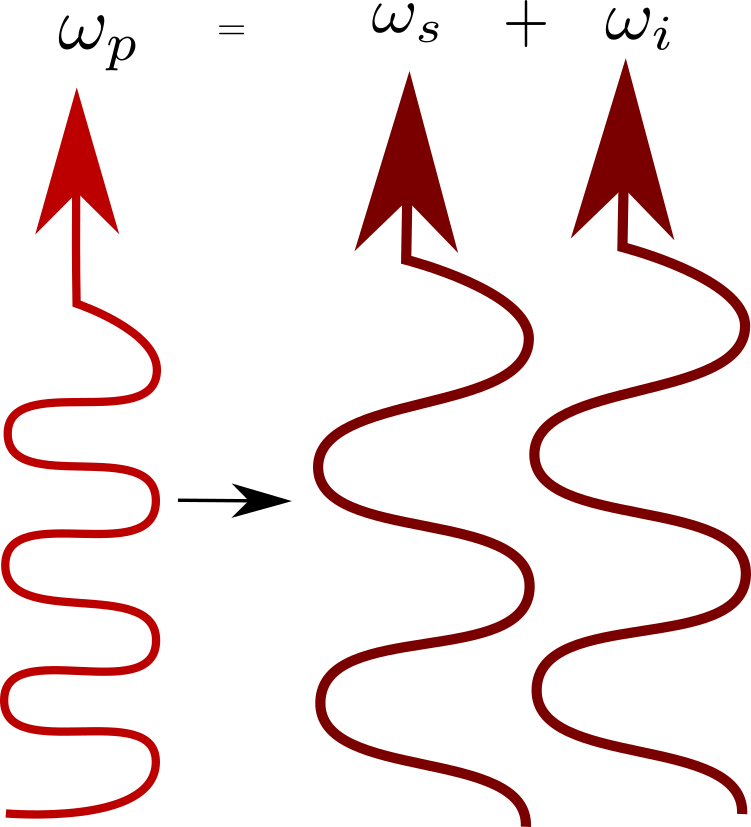
\includegraphics[width=4cm]{SPDC.png}
			\end{center}
			\caption{Illustration of SPDC}\label{fig:}
		\end{figure}
		\begin{itemize}
			\pause
			\item Asymmetric (non-degenerate)
			\item State of the art
			\item Different designs
		\end{itemize}
		
\end{frame}

\subsubsection{Phase Matching}
\begin{frame}
	\frametitle{SPDC}
	\framesubtitle{Phase Matching, Quasi Phase Matching, Bandwidth}
	\begin{itemize}
		\item Phase Matching, Quasi Phase Matching
	\end{itemize}
	\begin{equation}
	f(\text{T},\text{T0})\text{=}(T-\text{T0}) (T+\text{T0}+546.3)
		\label{eq:Temperature_Dependance}
	\end{equation}
	\begin{equation}
		\text{nS}(\text{a},\text{b},\text{T},\lambda)\text{=}\sqrt{ a_1+\text{f}\cdot b_1\frac{a_2+\text{f} \cdot b_2}{\lambda ^2-(a_3+\text{f} \cdot b_3)^2}+\frac{a_4+\text{f} \cdot b_4}{\lambda ^2-a_5^2}-a_6\lambda ^2}]
		\label{eq:Refractive_Index}
	\end{equation}
	\begin{itemize}
		\item Focusing parameters, Heralding,...
		\item Brightness
		\item Bandwidth
	\end{itemize}
\end{frame}

\begin{frame}[t]
	\frametitle{Type-II vs Type-0}
	\framesubtitle{Bandwidth}
	
	\begin{figure}[!ht]
	  \centering
	  \caption{Wavelength bandwidth of a) Type-2 crystal with a polling period of 9,12 um\\ Type-0 crystals with polling periods of b) 19,25 um}
	  \subfloat[][]{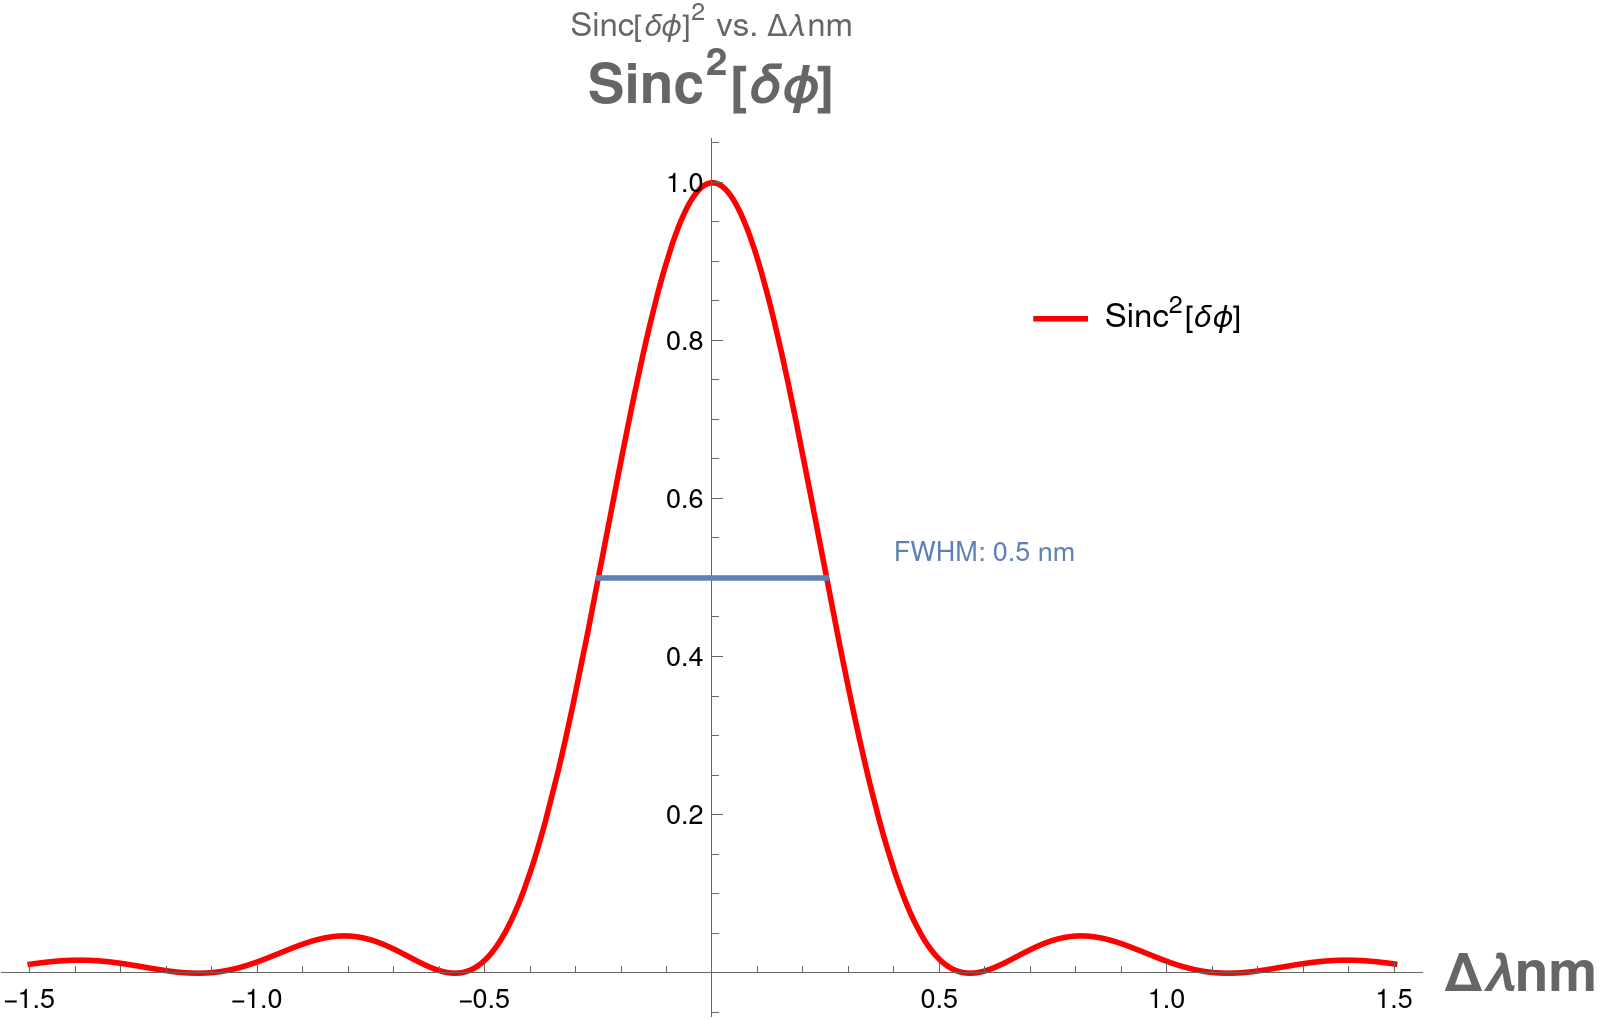
\includegraphics[width=5cm]{Type2wavelength.png}}\quad
	  \pause
	  \subfloat[][]{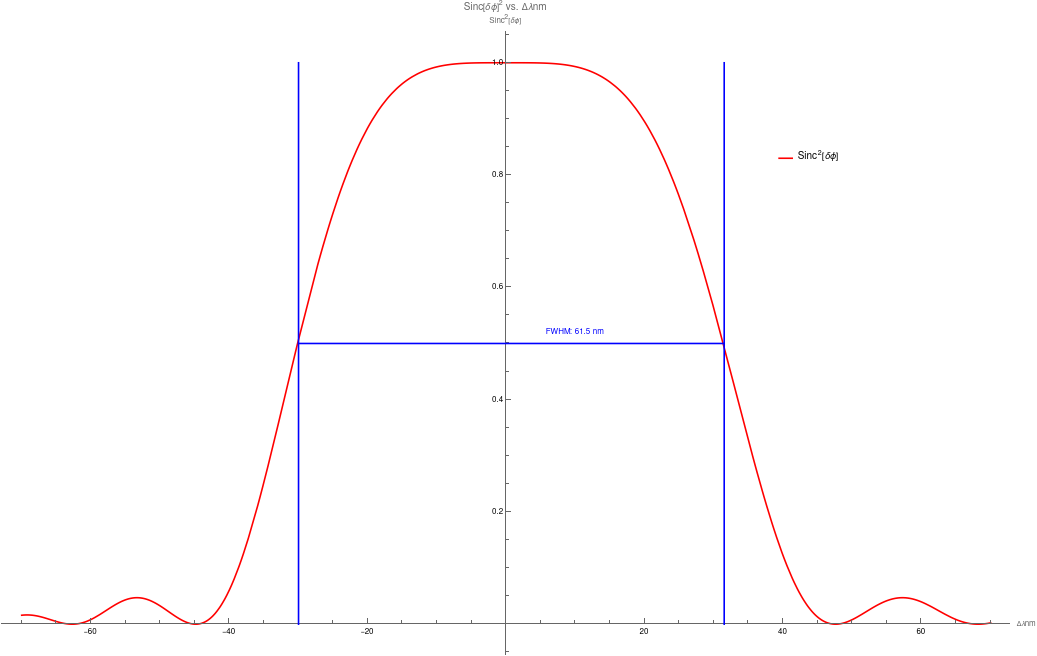
\includegraphics[width=5.5cm]{Type0wavelength.png}}
	  \label{fig:sub1}
	\end{figure}
\end{frame}

\begin{frame}
	\frametitle{SPDC}
	\framesubtitle{Type-2 vs Type-0}

	\begin{table}
		\begin{center}
		\caption{Brightness comparison \[Hz/mW/nm\]}
			\begin{tabular}[c|c|c]{|ll|l|}
				\hline
				\multicolumn{1}{|c}{\textbf{FMF}} & & 
				\multicolumn{1}{c|}{\textbf{IJS}} \\
				\hline 
				\multicolumn{1}{|c|}{\textbf{Type-II}} &
				\multicolumn{1}{c|}{\textbf{Type-0}} &
				\multicolumn{1}{c|}{\textbf{Type-II}} \\
				\hline
				7,8$\times10^6$ & 2,6$\times 10^7$ & 0,5$\times 10^6$\\
				\hline
			\end{tabular}
		\end{center}
	\end{table}

	\end{frame}

\subsubsection{Detectors}
\begin{frame}
	\frametitle{Detectors}
	\framesubtitle{Dependence of detector dead-time and efficiency}
Dead-time dependency
\end{frame}

\subsubsection{Efficiency}
\begin{frame}
	\frametitle{SPDC}
	\framesubtitle{Expected efficiency}
	Fiorentino
Expected efficiency
\end{frame}

\subsection{Entanglement swapping}
\begin{frame}{Entanglement swapping}
	\begin{itemize}
		\item FMF/IJS
		\item Quantum Repeaters
			\begin{enumerate}
				\item Quantum Memory - wrong wl for now, have to figure out
			\end{enumerate}
	\end{itemize}

\end{frame}

\section{Present state}

%Temperatures in the 100°C-200°C range are used in order to minimize the photorefractive effect that can damage the crystal and causes the output beam to be distorted.
%Since the photorefractive effect is more severe in PPLN when higher energy photons in the visible part of the spectrum are present in the crystal,
%it is especially important to use the crystal only in the recommended temperature range.
%When using a PPLN crystal as an OPO that is pumped with and generates light in the infrared region of the spectrum,
% it may be possible to use temperatures lower than 100°C if necessary without damaging the crystal.

\subsection{Implementations}
\begin{frame}[t]
	\frametitle{Present state}
	\framesubtitle{Building a linear test setup}

\end{frame}

\subsection{Phase Matching Temperature}
\begin{frame}{Present state}
	\framesubtitle{Phase Matching Temperature}
	\begin{figure}[!ht]
	  \centering
	  \caption{Temperature scans of Type-0 crystals with different polling periods, a) misaligned, b) 19,25 $\mu$m, c) 19,45 $\mu$m, d) 19,65 $\mu$m}
	  \subfloat[][]{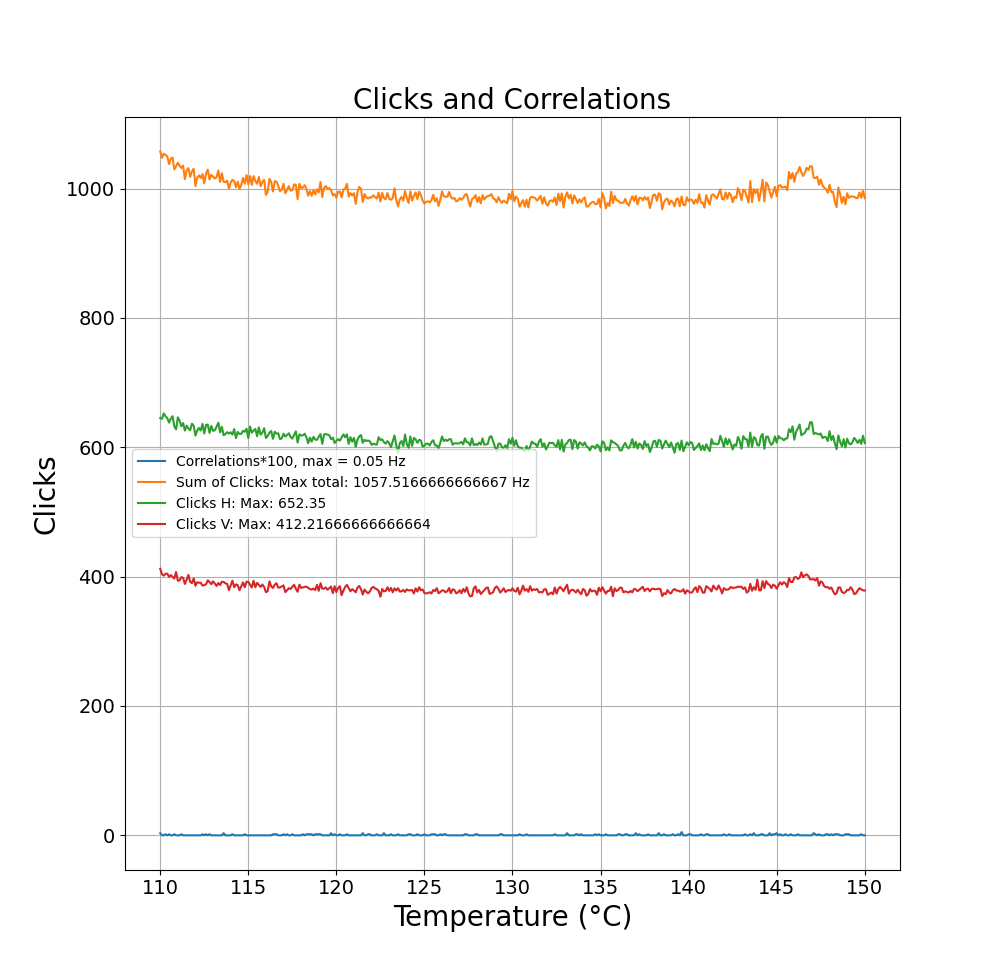
\includegraphics[width=2.9cm]{Not_Aligned_Scan.png}}\quad
	  \pause
	  \subfloat[][]{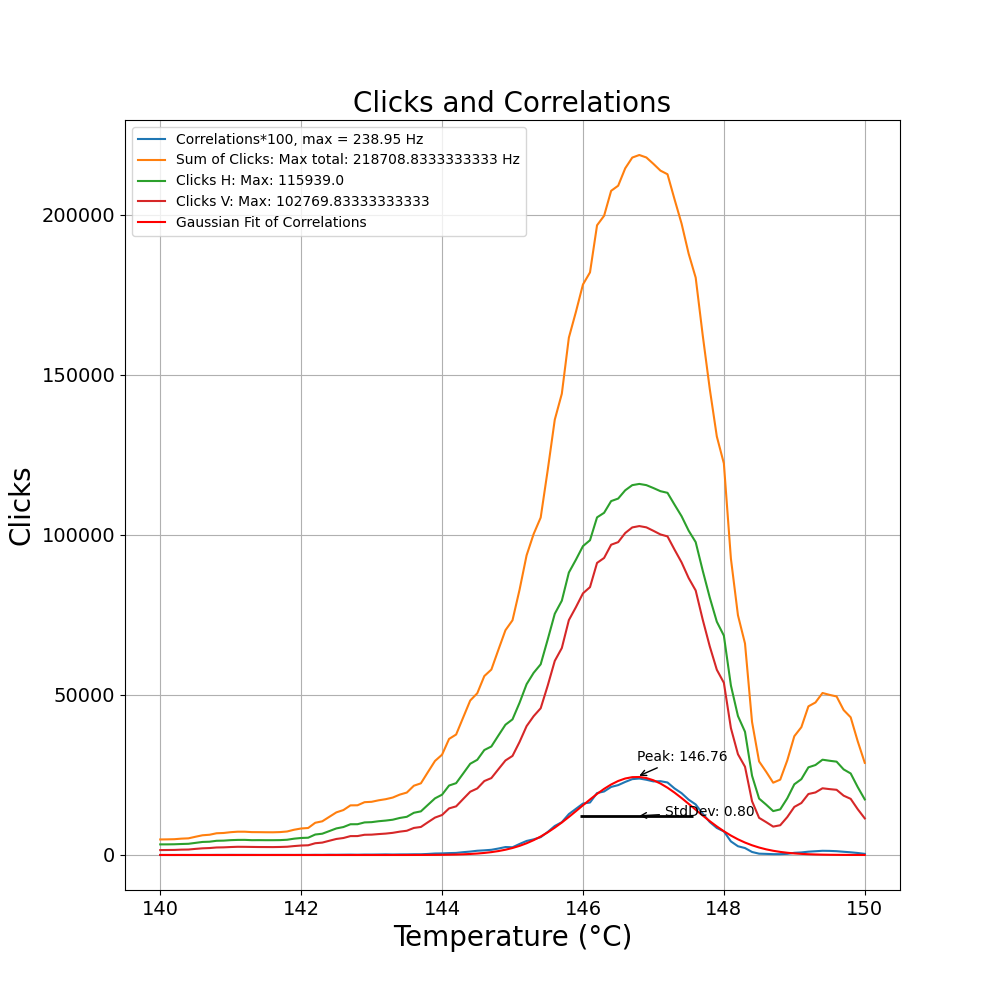
\includegraphics[width=2.9cm]{PMT_Grating_4.png}}\\
	  \subfloat[][]{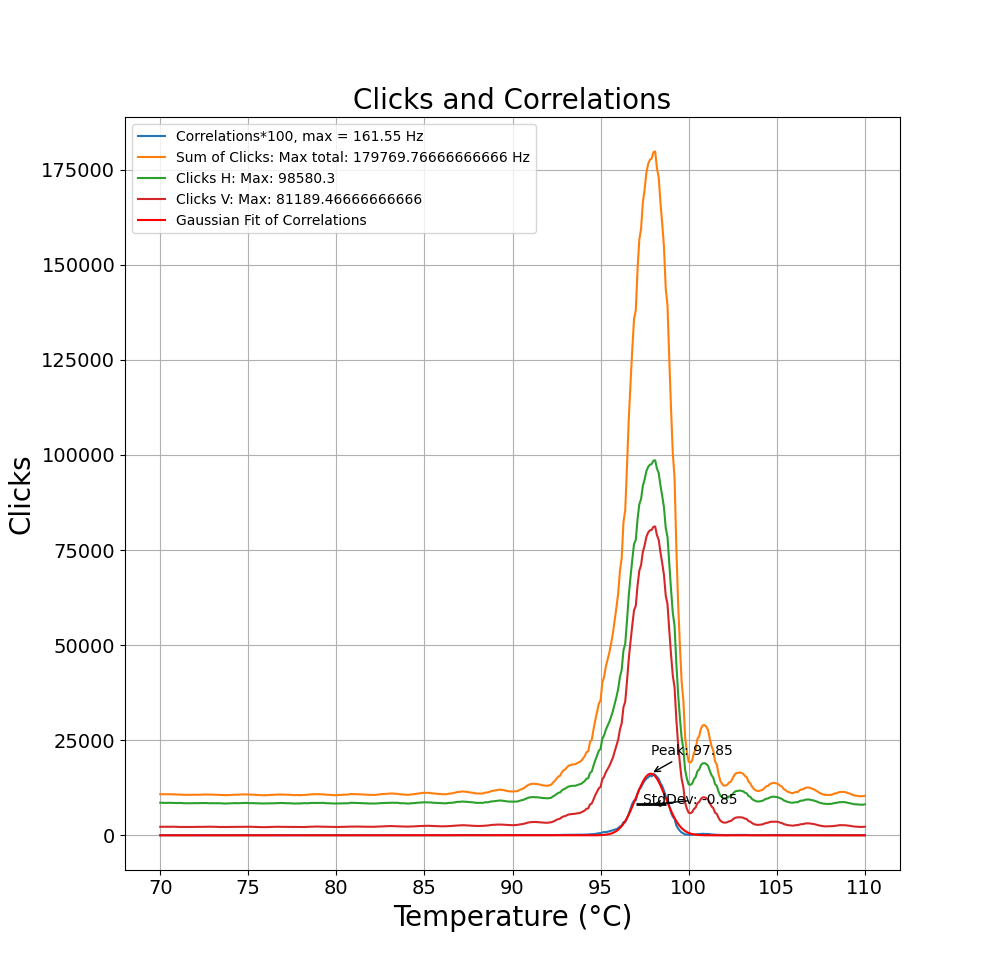
\includegraphics[width=2.9cm]{PMT_Grating_5.png}}\quad
	  \subfloat[][]{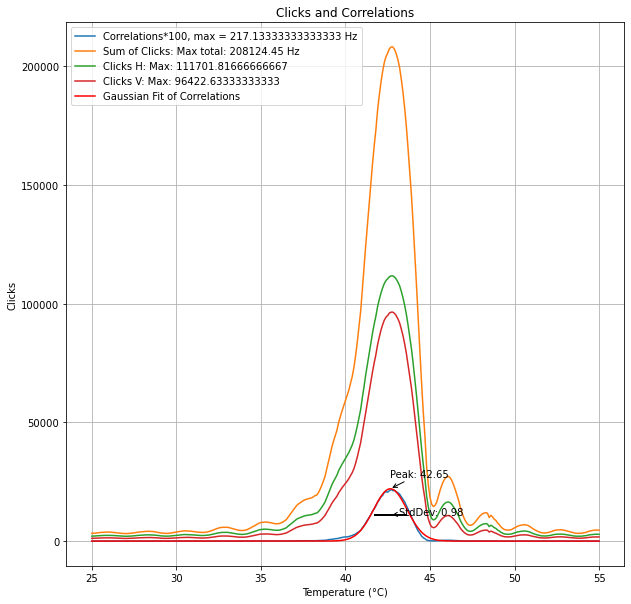
\includegraphics[width=2.9cm]{PMT_Grating_6.png}}\\
	  \label{fig:sub2}
	\end{figure}
\end{frame}

{\usebackgroundtemplate{\includegraphics[width=\paperwidth,height=\paperheight]{SagnacWithSomeAddedColoursV1.png}}
\begin{frame}[t]
	\frametitle{Present state}
	\framesubtitle{Building a Sagnac Interferometer}

	\begin{figure}[!ht]
	  \centering
	  % \subfloat[][]{\includegraphics[width=5cm]{SagnacWithSomeAddedColoursV1.png}}\quad
	  \pause
	  \subfloat[][]{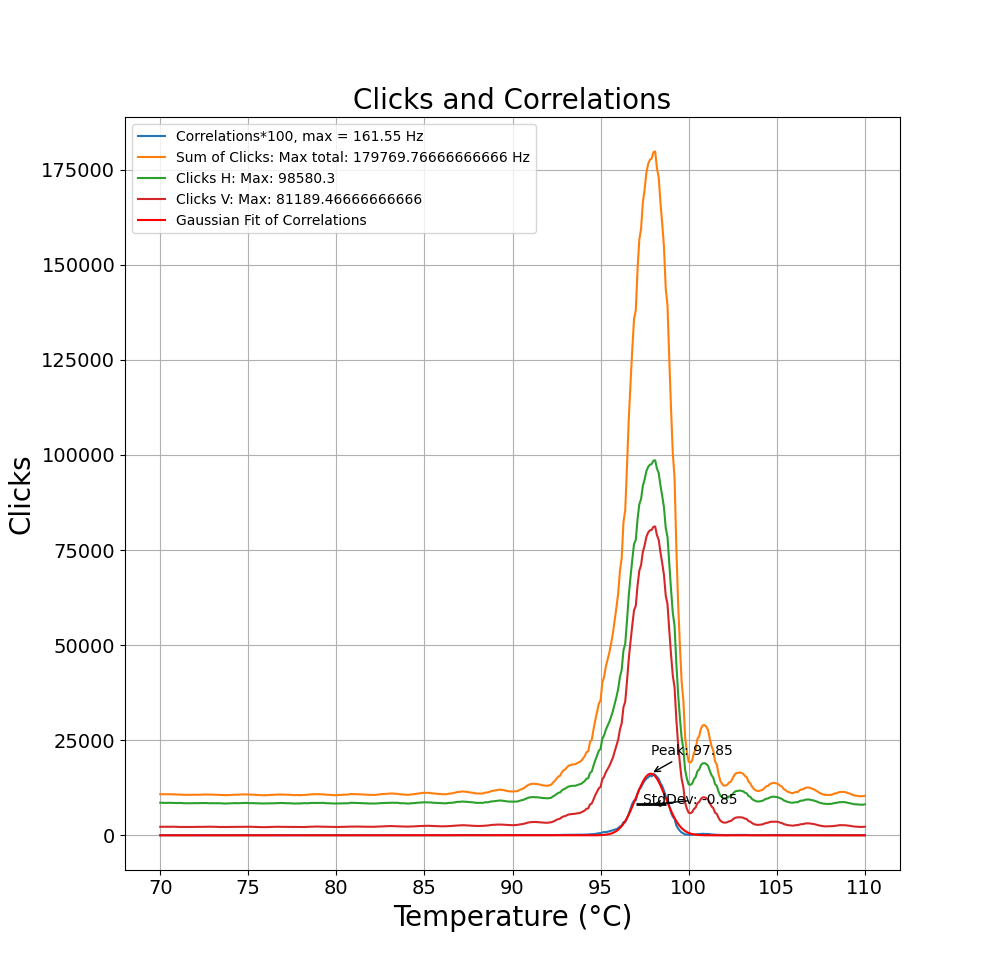
\includegraphics[width=5cm]{PMT_Grating_5.png}}\\
	\caption{3D design of the Sagnac interferometer}
	\end{figure}
\end{frame}

\usebackgroundtemplate{}
\section{Outlook}
\begin{frame}{Outlook}
	\begin{itemize}
		\item SiQUID
		\item Entanglement swapping between FMF and IJS
		\item Building quantum internet
	\end{itemize}
\end{frame}

\begin{frame}{Conclusion}
	\begin{center}
		\Large
		Testing, calculating various properties of the system, limitations, 
	\end{center}
\end{frame}

\begin{frame}{\ }
	\begin{center}
	\Huge
	Thank you
	\end{center}
\end{frame}

\end{document}
